%%%%%%%% ICML 2019 EXAMPLE LATEX SUBMISSION FILE %%%%%%%%%%%%%%%%%

\documentclass{article}

\usepackage[margin=1in]{geometry}
\usepackage{indentfirst}
% \usepackage{multibbl}


\usepackage[utf8]{inputenc} % allow utf-8 input
\usepackage[T1]{fontenc}    % use 8-bit T1 fonts
\usepackage{hyperref}       % hyperlinks
\usepackage{url}            % simple URL typesetting
\usepackage{booktabs}       % professional-quality tables
\usepackage{amsfonts}       % blackboard math symbols
\usepackage{nicefrac}       % compact symbols for 1/2, etc.
\usepackage{microtype}      % microtypography

\usepackage{bbm}
\usepackage{amsfonts}
\usepackage{amsmath,amsthm}           
\usepackage{mathtools}    
\usepackage{amsopn}
\usepackage{amssymb}
\usepackage{bm}
\usepackage{multirow}
\usepackage{graphicx}
\usepackage{subfigure}
% \usepackage{subcaption}
\usepackage{adjustbox}
\usepackage{xcolor}
\usepackage[vlined,linesnumbered,ruled]{algorithm2e}
\usepackage{biblatex}


\newcommand{\avgR}{\wh{\cal{R}}}
\newcommand{\ips}{\wh{r}}
\newcommand{\whpi}{\wh{\pi}}
\newcommand{\whE}{\wh{\E}}
\newcommand{\whV}{\wh{V}}
\newcommand{\Reg}{\text{\rm Reg}}
\newcommand{\SA}{\text{\rm SA}}
\newcommand{\whReg}{\wh{\text{\rm Reg}}}
\newcommand{\flg}{\text{\rm flag}}
\newcommand{\one}{\boldsymbol{1}}
\newcommand{\var}{\Delta}
\newcommand{\p}{\prime}
\newcommand{\nb}{\nabla}
\newcommand{\epo}{\text{epoch}}

\DeclareMathOperator*{\arginf}{arginf}
\DeclareMathOperator*{\argsup}{argsup}
\DeclareMathOperator*{\range}{range}
\DeclareMathOperator*{\mydet}{det_{+}}
\DeclarePairedDelimiter\abs{\lvert}{\rvert}
\DeclarePairedDelimiter\bigabs{\big\lvert}{\big\rvert}
\DeclarePairedDelimiter\ceil{\lceil}{\rceil}
\DeclarePairedDelimiter\floor{\lfloor}{\rfloor}
\DeclarePairedDelimiter\bigceil{\big\lceil}{\big\rceil}
\DeclarePairedDelimiter\bigfloor{\big\lfloor}{\big\rfloor}

\newcommand{\field}[1]{\mathbb{#1}}
\newcommand{\fY}{\field{Y}}
\newcommand{\fX}{\field{X}}
\newcommand{\fH}{\field{H}}
\newcommand{\fR}{\field{R}}
\newcommand{\fN}{\field{N}}
\newcommand{\E}{\field{E}}

\newcommand{\theset}[2]{ \left\{ {#1} \,:\, {#2} \right\} }
\newcommand{\inner}[1]{ \left\langle {#1} \right\rangle }
\newcommand{\Ind}[1]{ \field{I}_{\{{#1}\}} }
\newcommand{\eye}[1]{ \boldsymbol{I}_{#1} }
\newcommand{\norm}[1]{\left\|{#1}\right\|}
%\newcommand{\trace}[1]{\text{tr}\left({#1}\right)}
\newcommand{\trace}[1]{\textsc{tr}({#1})}
\newcommand{\diag}[1]{\mathrm{diag}\!\left\{{#1}\right\}}
\newcommand{\UB}{\text{UB}}
\newcommand{\defeq}{\stackrel{\rm def}{=}}
\newcommand{\sgn}{\mbox{\sc sgn}}
\newcommand{\scI}{\mathcal{I}}
\newcommand{\scO}{\mathcal{O}}
\newcommand{\scN}{\mathcal{N}}
\newcommand{\order}{\ensuremath{\mathcal{O}}}
\newcommand{\otil}{\ensuremath{\widetilde{\mathcal{O}}}}
% \newcommand{\Pr}{\ensuremath{\mathrm{Pr}}}

\newcommand{\dt}{\displaystyle}
\renewcommand{\ss}{\subseteq}
\newcommand{\wh}{\widehat}
\newcommand{\wt}{\widetilde}
\newcommand{\ve}{\varepsilon}
\newcommand{\hlambda}{\wh{\lambda}}
\newcommand{\yhat}{\wh{y}}

\newcommand{\hDelta}{\wh{\Delta}}
\newcommand{\hdelta}{\wh{\delta}}
\newcommand{\spin}{\{-1,+1\}}
\newcommand\numberthis{\addtocounter{equation}{1}\tag{\theequation}}

\newcommand{\mc}[1]{\mathcal{#1}}
\newcommand{\mb}[1]{\mathbb{#1}}
\newcommand{\mr}[1]{\mathrm{#1}}

%%%%%%%%%%%%%%%%%%%%%%%%

\newtheorem{assumption}{Assumption}
\newtheorem{theorem}{Theorem}
\newtheorem{lemma}{Lemma}
\newtheorem{corollary}[theorem]{Corollary}
\newtheorem{proposition}{Proposition}
\newtheorem{definition}{Definition}
\newtheorem{remark}{Remark}
\DeclareMathOperator{\val}{val}
\DeclareMathOperator{\spa}{sp}
\DeclareMathOperator{\solve}{solve}
\allowdisplaybreaks

% Packages hyperref and algorithmic misbehave sometimes.  We can fix
% this with the following command.
%\newcommand{\theHalgorithm}{\arabic{algorithm}}

\DeclareMathOperator*{\argmin}{\arg\!\min}
\DeclareMathOperator*{\argmax}{\arg\!\max}
% \setlength\parindent{10pt}

\newcommand{\compilefullversion}{true}%SHOW short version
\ifthenelse{\equal{\compilefullversion}{false}}{%
    \newcommand{\OnlyInFull}[1]{}
    \newcommand{\OnlyInShort}[1]{#1}
}{%
    \newcommand{\OnlyInFull}[1]{#1}%
    \newcommand{\OnlyInShort}[1]{}%
}%

% Macro for comments:
% \newcommand{\compilehidecomments}{false}%HIDE comments

% \ifthenelse{\equal{\compilehidecomments}{true}}{%
%     \newcommand{\wei}[1]{}
%     \newcommand{\haoyu}[1]{}
%     \newcommand{\kai}[1]{}
% }{
%     \newcommand{\wei}[1]{{\color{blue!50!black}  [\text{Wei:} #1]}}
%     \newcommand{\haoyu}[1]{{\color{brown!60!black} [\text{Haoyu:} #1]}}
%     \newcommand{\kai}[1]{{\color{purple} [\text{Kai:} #1]}}
% }


\allowdisplaybreaks

\title{Offline reinforcement learning with delay rewards}
\author{
xxx\\
Nanjing University\\
\texttt{xxx}
\and
xxx\\
Kuaishou Corp.\\
\texttt{xxx}
}
\date{}

\addbibresource{reference.bib}
% \newbibliography{main}
% \newbibliography{appendix}

\begin{document}
\maketitle

\begin{abstract}  
blablabla
\end{abstract}

\section{Introduction}

This is introduction part.




\section{Preliminaries}\label{sec:prel}
{\bf Notations:} $[p] = \{1,2,\cdots, p\}$. $d$ is the dimension of decision space, and $e_i$ represents $i$-th basis vector. For a vector $x$ and a matrix $M$, define $\norm{x}_M:=\sqrt{x^\top Mx}$. Given a set $\mc{W}$, we define the projection into this set as $\Pi_{\mc{W}}(\cdot)$. 




\section{Method}
In this section, we present a general framework for addressing sparse reward problems in offline setting. From a global perspective, the framework consists of two-stage learning tasks, in the first stage we perform specific transformation strategy on the offline datasets, and the second stage is a regular offline reinforcement learning task.

\textbf{Reward transformation.} Our key idea is to transmute the sparse delayed rewards into some dense instant rewards. Such transformation makes it possible to capture the meaningful patterns of original none-delayed rewards, 


\textbf{Offline policy optimization.}



\section{Experiments}

\subsection{Evaluation on d4rl datasets}

\textbf{Datasets construction.} In order to make a public comparison with other offline algorithms, we delay the dense reward based on the d4rl gym datasets. Specifically, we perform constant delay setting: we set a hyper-parameter $K$ as the delay interval which controls the sparsity of the delayed rewards. We set the delayed reward at equal intervals with $K$ as the un-discounted cumulative rewards of corresponding interval, the missing reward filled with 0, formally:

For a trajectory $\tau$ with length $T$, we set the delayed reward of time step $t$ as $r_t^{delay}$, where:

$$
\begin{aligned}
r_t^{delay} = \begin{cases}
0, \text{if} \ t \mod K \neq 0; \\
\sum_{i = t - K + 1}^t r_t, \text{otherwise}.
\end{cases}
\end{aligned}
$$

Such construction strategy introduce sparsity to delay rewards, meanwhile, it keeps the rule that for any trajectory in the original datasets, the un-discounted cumulative rewards keep constant before and after the operation, mathematically, we have:

$$
\sum_{t = 1}^{T} r_t = \sum_{t = 1}^{T} r_t^{delay}
$$

To facilitate intuitive and clear comparison of the delay reward construction method, visualization shows that:
\begin{figure}
    \centering
    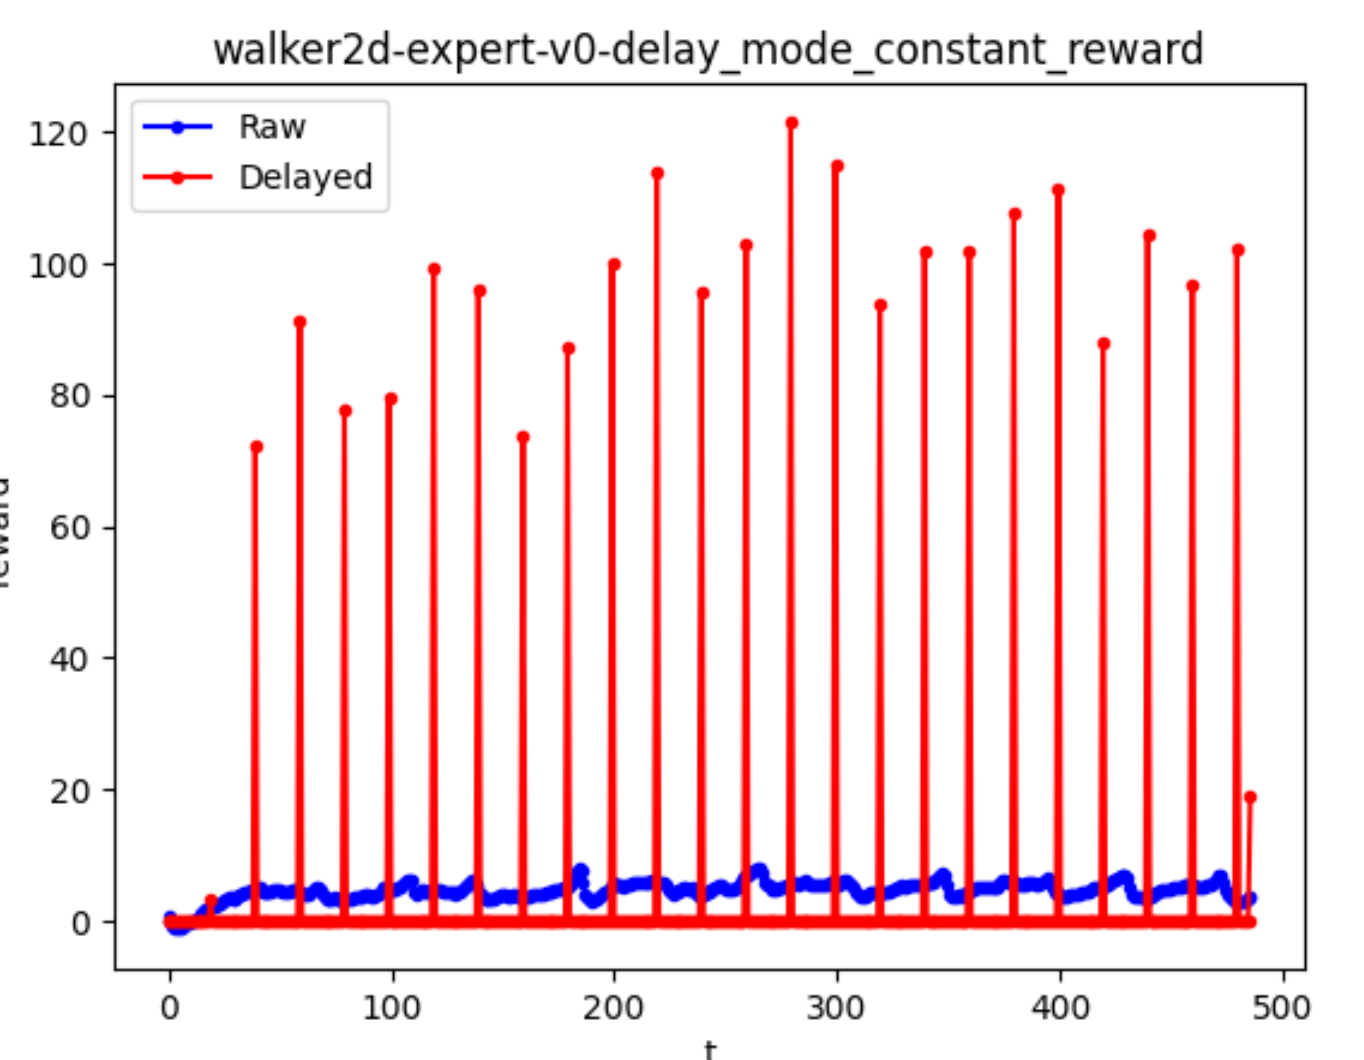
\includegraphics[width=0.95\textwidth]{assets/image.png}
    \caption{Delayed rewards xxx}
    \label{fig:fig1}
\end{figure}

\subsection{Evaluation on simulated datasets}


\subsection{Ablation Study}




\section{Conclusions}
In this paper, we propose a xxx.  



% \begin{ack}
% Use unnumbered first level headings for the acknowledgments. All acknowledgments
% go at the end of the paper before the list of references. Moreover, you are required to declare 
% funding (financial activities supporting the submitted work) and competing interests (related financial activities outside the submitted work). 
% More information about this disclosure can be found at: \url{https://neurips.cc/Conferences/2020/PaperInformation/FundingDisclosure}.


% Do {\bf not} include this section in the anonymized submission, only in the final paper. You can use the \texttt{ack} environment provided in the style file to autmoatically hide this section in the anonymized submission.
% \end{ack}

\newpage
% \bibliographystyle{abbrvnat}
% \bibliographystyle{plainnat}
% \bibliography{reference} 

\printbibliography

% \bibliographystyle{main}{plain}
% \bibliography{main}{reference}{reference}
   

\newpage
\appendix
% \begin{refsection}
\section*{Appendix}
\addcontentsline{toc}{section}{Appendices}
% \renewcommand{\thesubsection}{\Alph{subsection}}

\section{Reward Modification Implementation Details}
\label{appendix: rm_imp_details}
XXXX

\section{Experiment Details}
\label{appendix: exp_details}
Our implementation is based on the OfflineRL library released by NeoRL team.
For all experiments, we used default hyperparameter settings and minimal 
modifications to public implementations wherever possible, with different 
training iterations or gradient steps depending on the algorithm. We ran our 
experiments using single 1080 GPU machines.

\subsection{D4RL benchmark}\label{appendix: exp_d4rl_details}
XXX

\subsection{Custom simulated environment}\label{appendix: exp_custom_detials}
We build our simulated environment on the RecSim framework for its flexibility and scalability, RecSim is published by 
google research team to build a configurable platform for building simulated environments 
for recommender systems (RSs) that naturally supports sequential interaction with users.

Datasets are collected by pretraining an agent in Soft Actor-Critic way from scratch and collecting 1000 trajectories at 4 different levels:

\begin{itemize}
    \item Random: 
    \item Low: 
    \item Medium: 
    \item Expert:
\end{itemize}


% \printbibliography[heading=subbibliography]
% \end{refsection}

% \bibliographystyle{appendix}{plain}
% \bibliography{appendix}{reference}{reference}




\end{document}